\documentclass[a4paper, 12pt]{article}
\usepackage{amssymb}
\usepackage{amsmath}
\usepackage{tikz}
\usepackage{pgfplots}
\pgfplotsset{compat = newest}
\usepackage{multicol}
\usepackage{graphicx}
\graphicspath{ {./images/} }
\usetikzlibrary{calc}

\begin{document}

\title{Physics Beyond - Modelling Problems in Mechanics}
\author{Nathan Morris}
\maketitle

\newpage

\pagenumbering{roman}
\tableofcontents
\pagenumbering{arabic}

\newpage

\section{Modelling Problems in Mechanics}
\underline{Problem:} Knowing the interactions modelled by forces find the motion of a particle.\\
\underline{Analyse:}
$$\vec{a} = \frac{\vec{F}}{m}$$
\subsection{\underline{Q:} Link acceleration and position?}
\begin{eqnarray*}
\vec{a} &=& \ddot{\vec{x}}\\
\ddot{\vec{x}} &=& \frac{\vec{F}}{m}\vec{x}(t) \leftarrow \text{but $\vec{F}$ needs to depend on position!}\\
\vec{a}(t) &=& \ddot{\vec{x}}(t)\\
\end{eqnarray*}
$\rightsquigarrow$ Vector model fails!\\
replace with a vector field $\vec{F}$\\
$$\vec{F}: \text{positions $\rightarrow$ vectors}$$
$$x \rightarrow \vec{F}(x)$$
Use reference frame
$$ \vec{F} : R^3 \rightarrow R^3$$
$$ \vec{x} \mapsto \vec{F}(\vec{x})$$
\underline{Example:} Force of gravity (Close to Earth surface)
\begin{multicols}{2}
\begin{enumerate}
\item[1)] $$\ddot{\vec{x}} = \frac{m\vec{g}}{m} = \vec{g}$$
\item[2)] $$\ddot{\vec{x}} = \frac{M_{Earth}}{|\vec{x}(t) - \vec{x}_0|^3}$$ $x_0 = \text{centre of the earth}$
\end{enumerate}
in case of 1) $$\vec{g}:R^3 \rightarrow R^3, \vec{x} \mapsto \vec{g} \text{(Constant vector field)}$$
\begin{center}
\begin{tikzpicture}
\draw[->] (0,0)node[right]{O = centre of the Earth} -- (0,5)node[above]{$\vec{x}(t)$};
\draw[<->] (0.5,5) -- (0.5,3.5)node[right]{$\vec{F}_{grav}(\vec{x}(t))$};
\end{tikzpicture}
\end{center}
\end{multicols}
\begin{multicols}{3}
\begin{tikzpicture}
\draw[->] (0,6) -- (0,5);\draw[->] (0,4)node[left]{$\vec{g}$} -- (0,3);\draw[->] (0,2) -- (0,1);
\draw[->] (1,6)node[above]{Constant vector field} -- (1,5);\draw[->] (1,4) -- (1,3);\draw[->] (1,2) -- (1,1);
\draw[->] (2,6) -- (2,5);\draw[->] (2,4) -- (2,3);\draw[->] (2,2) -- (2,1);
\draw[->] (4,3) -- (4,4)node[left]{Z};\draw[->] (4,3,0) -- (4,3,1)node[above]{X};\draw[->] (4,3) -- (5,3)node[above]{Y};
\node (A) at (9,3) {O};
\draw[->] (8,3) -- (8.75,3); \draw[->] (7,3) -- (7.75,3);\draw[->] (6,3) -- (6.75,3);
\draw[<-] (9.25,3) -- (10,3); \draw[<-] (10.25,3) -- (11,3); \draw[<-] (11.25,3) -- (12,3);
\draw[<-] (9,2.75) -- (9,2);\draw[<-] (9,1.75) -- (9,1);\draw[<-] (9,0.75) -- (9,0);
\draw[<-] (9,3.25) -- (9,4);\draw[<-] (9,4.25) -- (9,5);\draw[<-] (9,5.25) -- (9,6);
\end{tikzpicture}
\end{multicols}
\subsection{\underline{Q:} What are we dealing with mathematically?}
$\rightarrow$ 2nd order differential equation
\begin{eqnarray*}
\vec{v}(t+dt) &=& \dot{\vec{x}}(t+dt)\\
&=& \dot{\vec{x}}(t) + \ddot{\vec{x}}(t)dt\\
&=& \vec{v}(t) + \dot{\vec{v}}(t)dt\\
(=) \vec{v}(t+dt) - \vec{v}(t) = \dot{\vec{v}}(t)dt\\
d\vec{v} = \dot{\vec{v}}(t)dt = \frac{\vec{F}(\vec{x}(t))}{m}dt
\end{eqnarray*} 
\subsection{\underline{Q:} How do we go about this?}
$\rightarrow$ Suppose we are given an initial position: $\vec{x}(t=0)=\vec{x_0}$
$$\dot{x}(t=0) = \vec{v_0}$$
\begin{enumerate}
\item[I)] \begin{eqnarray*}
\vec{v}(0+dt) &=& \vec{v}(0) + \dot{\vec{v}}(0)dt\\
&=& \vec{v_0} + \frac{\vec{F}(\vec{x}(0))}{m}dt\\
&=& \vec{v_0} + \frac{\vec{F}(\vec{x_0})}{m}dt\\
\end{eqnarray*}
\item[II)] \begin{eqnarray*}
\vec{x}(0+dt) &=& \vec{x_0} + \dot{\vec{x}}(0)dt\\
&=& \vec{x_0} + \vec{v_0}dt
\end{eqnarray*}
\item[III)] \begin{eqnarray*}
\vec{x}(0+dt+dt_2) &=& \vec{x}(0+dt) + \dot{\vec{x}}(dt)dt_2\\
&=& \vec{x_0} + \vec{v_0}dt+\vec{v_0}dt_2 + \frac{\vec{F}(\vec{x_0})}{m}dt dt_2\\
&=& \vec{x_0} + \vec{v_0}(dt+ dt_2) + \frac{\vec{F}(\vec{x_0})}{m}dt dt_2
\end{eqnarray*}
\end{enumerate}

\section{Solving Equations of motion}
\subsection{\underline{Method:} (for N particles)}
\begin{enumerate}
\item[1)] Free body diagram of each particle
\item[2)] Find the resultant forces
\item[3)] Set up equations of motion
\item[4)] Solve equations of motion
\end{enumerate}
1)\\ 
\begin{center}
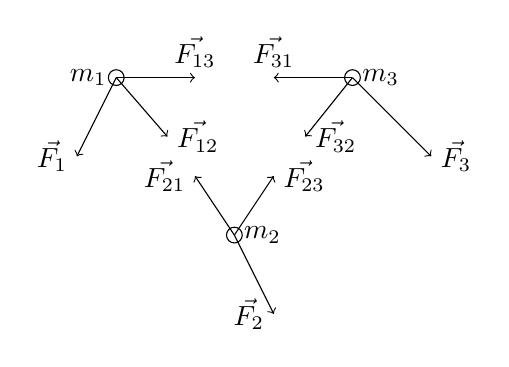
\begin{tikzpicture}
\draw (0,2) circle(0.1cm) node[left]{$m_1$};
\draw[->] (0,2) -- (0.65,1.25) node[right]{$\vec{F_{12}}$};
\draw[->] (0,2) -- (1,2) node[above]{$\vec{F_{13}}$};
\draw[->] (0,2) -- (-0.5,1) node[left]{$\vec{F_1}$};
\draw (1.5,0) circle(0.1cm) node[right]{$m_2$};
\draw[->] (1.5,0) -- (1,0.75) node[left]{$\vec{F_{21}}$};
\draw[->] (1.5,0) -- (2,0.75) node[right]{$\vec{F_{23}}$};
\draw[->] (1.5,0) -- (2,-1) node[left]{$\vec{F_2}$};
\draw (3,2) circle(0.1cm) node[right]{$m_3$};
\draw[->] (3,2) -- (2,2) node[above]{$\vec{F_{31}}$};
\draw[->] (3,2) -- (2.4,1.25) node[right]{$\vec{F_{32}}$};
\draw[->] (3,2) -- (4,1) node[right]{$\vec{F_3}$};
\end{tikzpicture}
\end{center}
2) Resultant force: $$\vec{F_i} = \sum_{f=1, i\neq j}^{N} \vec{F_{ij}} + \vec{F_{ext,i}} \text{ for all particles i}$$
3) $$m_i\ddot{\vec{x_i}} = \vec{F_i}$$
4) Task: find particles as a function of time $\vec{x_i}(t)$ for all particles based on the knowledge of forces.\\
$\rightarrow$ last time: force $\vec{F_{ij}}$ are modelled as vector fields. $$\vec{F_{ij}} : R^3 \times \mathbb{R}^3 \rightarrow \mathbb{R}^3$$
$$(\underbrace{\vec{x_i}}_{\text{Position of i-th particle}},\overbrace{\vec{x_j}}^{\text{Position of j-th particle}}) \mapsto \vec{F_{ij}}(\vec{x_i},\vec{x_j})\leftarrow \text{\parbox{6cm}{adding force on i-th particle due to j-th particles}}$$
$$m_i\ddot{\vec{x_i}} = \vec{F_i}(\vec{x_1},\cdots,No. \vec{x_i},\cdots,\vec{x_N})$$\\
\underline{Example:}
\subsection{Newton's law of gravity}
$$\vec{F_{EM}}(\vec{x_E},\vec{x_M})$$
\begin{eqnarray*}
F & = & G\frac{M_E M_M}{R^2}\\
& = &  \frac{GM_E M_M}{|\vec{x_M}-\vec{x_E}|^2} \cdot \frac{(\vec{x_M}-\vec{x_E})}{|\vec{x_M}-\vec{x_E}|}\\
& = & \frac{GM_E M_M}{|\vec{x_M}-\vec{x_E}|^3} \cdot (\vec{x_M}-\vec{x_E})\\
\end{eqnarray*}
Mathematically, the problem we are facing is to solve a system of 2nd order ordinary differential equation that is coupled.

\section{Ordinary Differential Equations(ODE):} 
\subsection{First Order Differential Equations}
\underline{Idea:} Flow of a river
****************River simulation.gif*****************
$\rightarrow$ Introduce a frame of reference\\
$$\vec{v}:R^2 \rightarrow \mathbb{R}^2$$
$$\overbrace{\vec{x}}^{\text{point on the river}} \mapsto \overbrace{\vec{v(\vec{x})}}^{\text{velocity at that point}}$$
$$\vec{x} : \overbrace{\mathbb{R}}^{\text{time}} \rightarrow \overbrace{\mathbb{R}^2}^{\text{position on the river}}$$
$$t \mapsto \vec{x}(t)$$
$$\dot{\vec{x}}(t) \text{velocity of leaf}$$
Since the leaf follows the flow of the river
$$\dot{\vec{x}}(t) = \vec{v}(\vec{x}(t))$$
First order differential equation
\subsection{ODE from an infinitesimal viewpoint}
\begin{multicols}{2}
\begin{center}
\begin{tikzpicture}
\draw[->] (0,0) node[below]{$\vec{x_0} = \vec{x}(t_0)$} -- (3,3)node[above]{$\vec{v}(\vec{x_0})$}node[right]{$\vec{x}(t+dt)$};
\end{tikzpicture}
\end{center}
$$\vec{x}(t_0 + dt) \overset{\text{kock - lawvere}}{=} \vec{x}(t_0) + \dot{\vec{x}}(t_0)dt$$
$$dt = D$$
according to ODE
\begin{eqnarray*}
\dot{\vec{x}}(t_0) &=& \vec{v}(\vec{x}(t_0))\\
&=& \vec{v(x_0)}
\end{eqnarray*}
\end{multicols}
$$\rightsquigarrow \vec{x}(t_0 + dt) = \vec{x_0} + \vec{v}(\vec{x_0})dt$$
$dt_1 , dt_2 \leftarrow D$
$$\vec{x}((t_0+dt_1)+dt_2) \overset{\text{K-L}}{=} \vec{x}(t_0 + dt_1) + \dot{\vec{x}}(t_0 + dt_1)dt_2$$
$$\text{ODE } \dot{\vec{x}}(t_0 + dt_1) = \vec{v}(\vec{x}(t_0 + dt_1))$$
$$ \vec{x}(t_0 + dt_1 + dt_2) = \vec{x}(t_0+dt_1) + \vec{v}(\vec{x}(t_0+dt_1))dt_2$$
$\rightarrow$ Iterating this method leads to what is called the infinitesimal \underline{Euler method.}
\subsection{Numerical Euler Method}
Instead of infinitesimal time steps $dt\leftarrow D$, use finite but small time steps,$\Delta t>0$.
\begin{center}
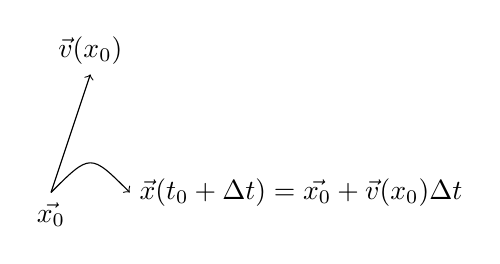
\begin{tikzpicture}
\draw[->] (0,0)node[below]{$\vec{x_0}$} -- (0.5,1.5)node[above]{$\vec{v}(x_0)$};
\draw[->] (0,0) .. controls (0.5,0.5) .. (1,0) node[right]{$\vec{x}(t_0 + \Delta t) = \vec{x_0} + \vec{v}(x_0) \Delta t$};
\end{tikzpicture}
\end{center}
This allows you to find an approximate solution $\vec{x}(t)$ of the 1st order ODE $\dot{\vec{x}} = \vec{v}(x)$
\subsubsection{Method:}
\begin{enumerate}
\item[1)] $$\vec{x}(t_0) = \vec{x_0} \text{(initial conditions)}$$
\item[2)] $$t_1 = t_0 + \Delta t$$ $$ \vec{x}(t_1) = \vec{x}(t_0 + \Delta t) = \vec{x}(t_0) + \vec{v}(\vec{x}(t_0)) \Delta t$$
\item[3)] after time $$t_n$$ $$t_{n+1} = t_n + \Delta t$$ $$\vec{x}(t_{n+1}) = \vec{x}(t_n) + \vec{v}(\vec{x}(t_n))\Delta t$$
\end{enumerate}

\section{1st Order ODEs from the differential point of view}
\subsection{Consider ODE}
$$ \text{for } v:\overbrace{R^n}^{\text{point}} \rightarrow \overbrace{R^n}^{\text{Velocity vector at point}}$$
$$ \dot{x} = v(x)$$
i.e we are looking for a curve/trajectory $x:R\rightarrow R^n, t \mapsto x(t)$
$$\dot{x}(t) = v(x(t))$$
for a solution to be uniquely determined we need an initial value $x(t_0) = x_0$
\subsection{Infinitesimal point of view}
for an infinitesimal time: $dt$ and $dx$ are \underline{both} infinitesimal differences.\\
for $dt \leftarrow D$
$$ x(t+dt) \overset{\text{K-L}}{=} x(t) + \dot{x}(t)dt $$
$$\Rightarrow \underbrace{x(t+dt) - x(t)}_{dx} = \dot{x}(t)dt$$
This is the differential of $x$ ($dx$), it is the infinitesimal displacement along $x(t)$.\\
(Reminder from multivariable calculus $dx \leftarrow D(n)$)\\
Using this notation and substituting ODE we find:
$$ dx = v(x)dt$$
$\rightsquigarrow$ an \underline{equation between differentials.}\\
$\rightsquigarrow$ strategy to find the \underline{finite} difference in displacement:
$$ \Delta x = x(t) - x(t_0)$$ from the differential equation we have to sum up all the infinitesimal displacements $dx = v(x)dt$ along the curve $x(t)$.
\begin{center}
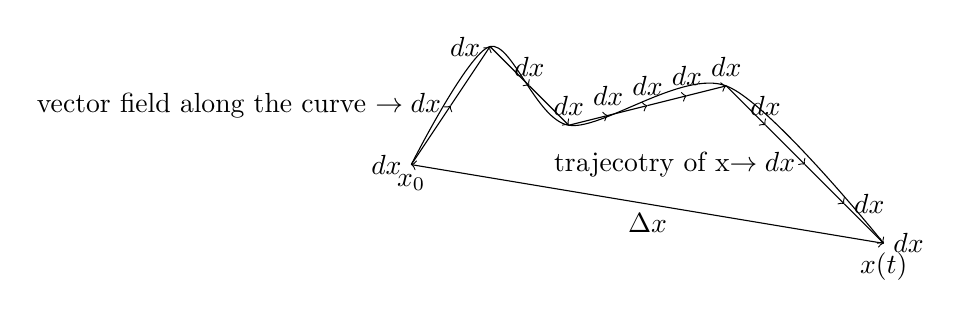
\begin{tikzpicture}
\draw plot[smooth] coordinates{(0,2)(1,3.5)(2,2.5)(4,3)(6,1)};
\draw[<-] (0,2) node[below]{$x_0$} -- (3,1.5)node[below]{$\Delta x$};
\draw[->] (3,1.5) -- (6,1)node[below]{$x(t)$};
\draw[->] (0,2)node[left]{$dx$} -- (0.5,2.75) node[left]{vector field along the curve $\rightarrow dx$};
\draw[->](0.5,2.75) --  (1,3.5)node[left]{$dx$};
\draw[->]  (1,3.5) -- (1.5,3)node[above]{$dx$};
\draw[->] (1.5,3) -- (2,2.5)node[above]{$dx$};
\draw[->]  (2,2.5) --  (2.5,2.625)node[above]{$dx$};
\draw[->](2.5,2.625) -- (3,2.75)node[above]{$dx$};
\draw[->](3,2.75) -- (3.5,2.875)node[above]{$dx$};
\draw[->] (3.5,2.875) -- (4,3)node[above]{$dx$};
\draw[->] (4,3) -- (4.5,2.5)node[above]{$dx$};
\draw[->] (4.5,2.5) -- (5,2)node[left]{trajecotry of x$\rightarrow dx$};
\draw[->] (5,2) -- (5.5,1.5)node[right]{$dx$};
\draw[->] (5.5,1.5) -- (6,1)node[right]{$dx$};
\end{tikzpicture}
\end{center}
\underline{Integration:}(Here along the curve!)\\
Is the idea to sum up all the infinitely many infinitesimal contributions (here along a curve) to get a finite result.
$$\text{stands for s like \underline{sum}} \rightarrow \int_{x_0}^{x(t)} dx = \int_{t_0}^{t} v(\tau)d\tau$$
need to develop a theory of integration sufficiently strong to integrate vector-valued infinitesimal contributions.
\subsection{Theory of integration from the infinitesimal viewpoint}
\underline{Basic Probelm:}
\begin{center}
\begin{tikzpicture}
\draw[->] (-1,0) -- (2.5,0)node[above]{A} --  (6,0);
\draw[->] (0,-1) -- (0,4);
\draw plot[smooth]coordinates{(-1,-1)(1,3)(3,1)(6,4)}node[right]{$f$};
\draw (1,3) -- (1,0) node[below]{a};
\draw (4,1.75) -- (4,0) node[below]{b};
\draw (7,2) -- (9,3) node[above]{Zoom};
\draw (7,2) -- (9,1);
\draw (10,0) -- (13,0);
\draw plot[smooth]coordinates{(10,2.75)(11,3)(13,2.5)};
\draw[dotted] (11,3) -- (11,0) node[below]{$a$};
\draw[dotted] (11.5,2.9)node[above]{$f(x)$} -- (11.5,0) node[below]{$x$};
\draw[dotted] (12.5,2.9)node[right]{$f(x+dx)$} -- (12.5,0)node[below]{$x+dx$};
\draw[dotted] (11.5,2.9) -- (12,2.9) node[above]{1} -- (12.5,2.9);
\draw[dotted] (11.5,2.6) -- (12,2.6) node[below]{2} -- (12.5,2.6);
\draw[dotted] (11.5,2.9) -- (12,2.75) node[left]{3} -- (12.5,2.6);
\end{tikzpicture}
\end{center}
Area of rectangle 1: $dA = f(x)dx$\\
Area of rectangle 2: $dA = f(x+dx)dx = (f(x) + f'(x)dx)dx = f(x)dx$\\
Area of trapezium 3: $dA = \frac{1}{2}(f(x) + f(x+dx))dx = \frac{1}{2}(f(x) + f(x) + f'(x)dx)dx = f(x)dx$\\
\underline{Q:} How to define\\
$$ A = \int_{a}^{b} dA = \int_{a}^{b} f(x)dx ?$$
$\rightsquigarrow$ problem: are not able to give a \underline{direct} \underline{intuitive} definition, as the theory has not been developed so far!\\
\underline{Q:} Can you find a way to \underline{evaluate} $ \int_{a}^{b} f(x)dx $ and use that as an \underline{effective} definition?\\
Observation:\\
$$ F(x+dx) \overset{\text{K-L}}{=} F(x) + F'(x)dx $$
$$ F(x+dx) - F(x) = F'(x)dx$$
Suppose I can find $F:R \rightarrow R$ such that $ F'(x) = f(x), vx \leftarrow R$ then I get $ F(x+dx) - F(x) = F'(x)dx = f(x)dx$.
\begin{center}
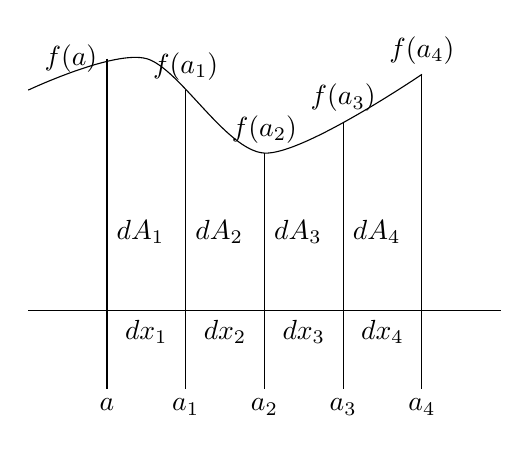
\begin{tikzpicture}
\draw (-1,0) -- (0.5,0)node[below]{$dx_1$} -- (1.5,0)node[below]{$dx_2$} -- (2.5,0)node[below]{$dx_3$} -- (3.5,0)node[below]{$dx_4$} -- ( 5,0);
\draw plot[smooth]coordinates{(-1,2.8) (0.5,3.2) (2,2) (4,3)};
\draw (0,3.2)node[left]{$f(a)$} -- (0,1)node[right]{$dA_1$} -- (0,-1)node[below]{$a$};
\draw (1,2.8)node[above]{$f(a_1)$} -- (1,1)node[right]{$dA_2$} --  (1,-1)node[below]{$a_1$};
\draw (2,2)node[above]{$f(a_2)$} -- (2,1)node[right]{$dA_3$} --  (2,-1)node[below]{$a_2$};
\draw (3,2.4)node[above]{$f(a_3)$} -- (3,1)node[right]{$dA_4$} -- (3,-1)node[below]{$a_3$};
\draw (4,3)node[above]{$f(a_4)$} -- (4,-1)node[below]{$a_4$};
\end{tikzpicture}
\begin{eqnarray*}
\text{Total Area} &=&dA_1 + dA_2 + dA_3 + dA_4 + ... \\
& = & f(a)dx_1 + f(a_1)dx_2 + f(a_2)dx_3 + f(a_3)dx_4 + ...\\
& = & F(a_1) - F(a) + F(a_2) - F(a_1) + F(a_3) - F(a_2) + F(a_4) - F(a_3)\\
& = & F(a_4) - F(a)\\ 
\end{eqnarray*}
\end{center}
\underline{Idea:} No matter how you would define an infinite sum of infinitesimals this cancellation process when summing up $$f(x)dx = dF = F(x+dx) - F(x)$$ should only depend on the boundary values.\\
(Fudge)\underline{definition:} $$ \int_{a}^{b} f(x)dx = F(b) - F(a) \text{ for an \underline{antiderivative} } F:R \rightarrow R \text{ of } f$$
\underline{Q:} How do we know an antiderivative exists?\\
$\rightarrow$ we don't, so we postulate it in the theory.
\subsection{Integration axiom}
\begin{itemize}
\item For every $f: R \rightarrow R$ there is an antiderivative $F:R \rightarrow R$, i.e $F' = f$
\item If $F$ and $F$ are antiderivatives of $f$ then $F - F$ is a constant function
\end{itemize}
Why difference constant?
\begin{multicols}{2}
\begin{tikzpicture}
\draw (0,1) --  (0,3)node[right]{$1$} -- (0,4)node[left]{$2$};
\draw (-2.5,2) -- (-2,2)node[below]{$-2$} -- (-1,2)node[below]{$-1$} -- (1,2)node[below]{$1$} -- (2,2)node[below]{$2$} -- (2.5,2);
\draw (-2,3) -- (-1,3);
\draw (1,3) -- (2,3);
\draw (0,-1)node[left]{$4$} --  (0,-2)node[right]{$1$} -- (0,-5)node[left]{$2$};
\draw (-2.5,-3) -- (-2,-3)node[below]{$-2$} -- (-1,-3)node[below]{$-1$} -- (1,-3)node[below]{$1$} -- (2,-3)node[below]{$2$} -- (2.5,-3);
\draw (-2,-5) -- (-1,-4);
\draw (1,-2) -- (2,-1);
\end{tikzpicture}
\vfill \null
$$ f: [-2,1] \cup [1,2] \rightarrow R$$
\begin{equation*}
f(x) = 
\begin{cases}
1, -2 \leq x \leq 1 \\
2, 1 \leq x \leq 2
\end{cases}
\end{equation*}
$$ F_1: [-2,1] \cup [1,2] \rightarrow R$$
\begin{equation*}
x \mapsto 
\begin{cases}
x, -2 \leq x \leq 1 \\
2x, 1 \leq x \leq 2
\end{cases}
\end{equation*}
$$ F_2: [-2,1] \cup [1,2] \rightarrow R$$
\begin{equation*}
x \mapsto 
\begin{cases}
x+4, -2 \leq x \leq 1 \\
2x-10, 1 \leq x \leq 2
\end{cases}
\end{equation*}
\end{multicols}
We have $F'_2 = f$ but $F_2(x) - F_1(x) = \begin{cases} 4, -2 \leq x \leq 1\\ -10, 1 \leq x \leq 2 \end{cases}$ is \underline{not} constant.\\
intuition: (has gaps)\\
On a domain that is `connected' the antiderivatives do not have to differ by a constant!
\subsection{Differentiation rules}
\subsubsection{Linearity} $$(f+g)' = f' + g' \text{(pointwise sum)}$$ $$(f+g)'(x) = f'(x) +g'(x)$$ $$(\lambda f)' = \lambda f'$$ $$(\lambda f)'(x) = \lambda f'(x)$$
\subsubsection{Product Rule} $$(f\cdot g)' = f' \cdot g + f \cdot g' \text{(pointwise product)}$$ $$ (f \cdot g)(x) = f(x)\cdot g(x)$$ $$(f\cdot g)'(x) = f'(x) \cdot g(x) + f(x) \cdot g'(x)$$
\subsubsection{Chain Rule} $$(f \circ g)' = (f' \circ g)'$$ $$(f \circ g)(x) = f(g(x))$$ $$(f \circ g)'(x) = f'(g(x))\cdot g'(x)$$
\subsection{Integration rules} 
\subsubsection{additivity} $$\int_{a}^{c} f(x) dx + \int_{c}^{b} f(x) dx  = \int_{a}^{b} f(x) dx$$ \underline{Proof:} 
\begin{eqnarray*}
 F(x) &=& \int f(x) dx\\
 &=& [F(x)]^c_a + [F(x)]^b_c\\
 &=& F(c) - F(a) +F(b) - F(c)\\
 &=& F(b) - F(a)\\
 &=& \int_{a}^{b} f(x) dx
 \end{eqnarray*}
\subsubsection{linearity} $$\int_{a}^{b} \lambda f(x) + g(x) dx = \lambda \int_{a}^{b} f(x) dx + \int_{a}^{b} g(x) dx$$ \underline{Proof:} 
\begin{eqnarray*}
\int_{a}^{b} \lambda f(x) + g(x) dx &=& \\
&=& [\int \lambda f(x) + g(x) dx]_{a}^{b}\\
&=& [\int \lambda f(x) + g(x) dx]^{b} - [\int \lambda f(x) + g(x) dx]_{a}\\
&=& [\int \lambda f(x) dx]^{b} - [\int \lambda f(x) dx]_{a} + [\int g(x) dx]^{b} - [\int g(x) dx]_{a}\\
&=& [\int \lambda f(x) dx]^{b}_{a} + [\int g(x) dx]^{b}_{a}\\
&=& \lambda[\int f(x) dx]^{b}_{a} + \int^{b}_{a} g(x) dx\\
&=& \lambda \int_{a}^{b} f(x) dx + \int_{a}^{b} g(x) dx
\end{eqnarray*}
\subsubsection{partial differentiation} $$\int_{a}^{b} f'(x)g(x) dx = [f(x)g(x)]_{a}^{b} - \int_{a}^{b} f(x)g'(x) dx$$ \underline{Proof:}
\begin{eqnarray*}
\text{Intergrate product rule: } (f\cdot g)'(x) = f'(x) \cdot g(x) + f(x) \cdot g'(x)\\
\int^{b}_{a}(f\cdot g)'(x)dx = \int^{b}_{a}f'(x) \cdot g(x) dx + \int^{b}_{a}f(x) \cdot g'(x) dx\\
\big[ (f\cdot g)(x)\big]^{b}_{a} = \int^{b}_{a}f'(x) \cdot g(x) dx + \int^{b}_{a}f(x) \cdot g'(x) dx\\
\rightsquigarrow \int^{b}_{a}f'(x) \cdot g(x) dx = [(f\cdot g)(x)]^{b}_{a} - \int^{b}_{a}f(x) \cdot g'(x) dx
\end{eqnarray*} \underline{Example:}
\begin{eqnarray*}
\int^{1}_{0} x sin(x) dx &=& \int^{1}_{0} g(x) f'(x) dx\\
&=& [-cos(x) \cdot x]^{1}_{0} - \int^{1}_{0} -cos(x) \cdot 1 dx\\
&=& -cos(1) + 0 + \int^{1}_{0} cos(x) dx\\
&=& -cos(1) + sin(1) - sin(0)\\
&=& sin(1) - cos(1)
\end{eqnarray*}
\subsubsection{substitution rule} $$\int_{a}^{b} f(g(x)) \cdot g'(x) dx = \int_{g(a)}^{g(b)} f(u)du$$ 
I do the substitution $u = g(x)$
$$du = g(x+dx) - g(x) = g(x) + g'(x)dx - g(x) = g'(x)dx$$
\underline{Example:}
\begin{eqnarray*}
\int_{0}^{1} sin(x^2) 2x dx, u=x^2, (x^2)^1 = 2x\\
&=& \int_{0}^{1} sin(u)du\\
&=& [-cos(u)]_{0}^{1} = cos(0) - cos(1) = 1 - cos(1)
\end{eqnarray*}
\underline{Example:}
Let $F$ be an antiderivative of $f$ $(F' = f)$ (Exists due to integration axiom)\\
Consider  $(F \circ g)' = F'\circ g\cdot g' = f \circ g \cdot g'$\\
$\rightsquigarrow F\circ g$ is the antiderivative of $f \circ g$
$$\rightsquigarrow\int^{b}_{a}(f(g(x))g'(x)dx = F(g(b)) - F(g(a)) = \int^{g(b)}_{g(a)} f(u) du \text{ (by definition)}$$
\underline{Remark:} Although the proof of integration by substitution is straight forward with the definitions we made, \underline{geometrically} it is \underline{not} straight forward.\\
\begin{tikzpicture}
\draw[->] (-1,0) -- (5,0)node[right]{$u$}; \draw[->] (0,-1) -- (0,4) node[left]{$y$};
\draw[->] (6,0) -- (12,0)node[right]{$x$}; \draw[->] (7,-1) -- (7,4) node[left]{$u$};
\draw plot[smooth] coordinates{(-1,1.5)(0,2)(2,1.75)(3,1.5)(5,2)}node[below]{$f$};
\draw[-] (1,1.875) -- (1,0) node[below]{$g(a)$}; \draw[-] (4,1.75) -- (4,0) node[below]{$g(b)$};
\draw[dotted] (2,1.75) -- (2,0) node[below]{$u$}; \draw[dotted] (3,1.5) -- (3,0) node[below]{$u+du$};
\draw plot[smooth] coordinates{(6,1.5)(7,2)(9,2.5)(10,2)(12,3)}node[right]{$g$};
\draw[dotted] (10,2) -- (7,2) node[left]{$u=g(x)$}; \draw[dotted] (11,2.5) -- (7,2.5) node[left]{$u+du=g(x)+dx$};
\draw[dotted] (10,2) -- (10,0)node[below]{$x$}; \draw[dotted] (11,2.5) -- (11,0)node[below]{$x+dx$}; 
\end{tikzpicture}
\underline{Q:} What if $g(x) = g(x+dx)$? (i.e. $x$ is a stationary point)\\
$\rightsquigarrow du=0$, but $dx$ is not probably equal to $0$.\\
This is not a problem as:$$du = g'(x)dx \text{ and } g'(x) = 0$$
\underline{Note:}
$$ \int^{a}_{a} f(x) dx = F(a) - F(a) = 0$$
$$ \int^{a+d}_{a} f(x) dx = F(a+d) - F(a) = f(a)d \text{ (K-L)}$$

\section{Vector Valued Integration}
\underline{Reminder:} For ODEs we had to consider $$dx = v(x) dt$$
\subsection{\underline{Q:} How do we link this back to the integral we just discussed?}
$\rightsquigarrow$ Introduce coordinates\\ 
Assume $x:R \rightarrow R^n$ is the solution to our ODE $dx = v(x)dt$\\
$$dx = x(t+dt) - x(t) = \dot{x}(t)dt = v(x(t))dt$$
$$x(t) = 
\begin{pmatrix}
x_1(t)\\
\vdots \\
x_n(t)
\end{pmatrix}$$
$$dx =
\begin{pmatrix}
x_1(t+dt) - x_1(t)\\
\vdots \\
x_n(t+dt) - x_n(t)
\end{pmatrix}
=
\begin{pmatrix}
v_1(x_1(t)& \cdots & x_n(t))dt \\
\vdots & \ddots & \vdots\\
v_n(x_1(t)& \cdots & x_n(t))dt
\end{pmatrix}$$
$\rightsquigarrow$ we can sum up the infinitely many infinitesimal vectors $v(x(t))dt$\\
in 1D summing over $f(x)dx$ , $v(x(t))dt$\\
\subsection{\underline{Definition:} (vector valued integral)}
$$ \gamma : R \rightarrow R^n, t \mapsto \gamma(t) = \begin{pmatrix} \gamma_1 (t)\\ \vdots \\ \gamma_n (t) \end{pmatrix} \text{(a curve)}$$
$$\int_{t_0}^{t_n} \gamma (t) dt = \begin{pmatrix} \int_{t_0}^{t_n} \gamma_1 (t) dt \\ \vdots \\ \int_{t_0}^{t_n} \gamma_n (t) dt \end{pmatrix}$$
\subsection{\underline{Q:} Is that well defined?}
Let $T_j : R \rightarrow R$ be the antiderivative of $\gamma_j$ for all $ 1 <= j <= n$\\
Consider $T : R \rightarrow R^n$ , $t \mapsto  \begin{pmatrix} T_1 (t)\\ \vdots \\ T_n (t) \end{pmatrix} \text{(a curve)}$
$$ \dot{T} (t) = \begin{pmatrix} \dot{T}_1 (t)\\ \vdots \\ \dot{T}_n (t) \end{pmatrix} =  \begin{pmatrix} \gamma_1 (t)\\ \vdots \\ \gamma_n (t) \end{pmatrix} = \gamma(t)$$
$\rightsquigarrow$ $T$ is an antiderivative for $\gamma$.
$$\int_{t_0}^{t_1} \gamma (t) dt = T(t_1) - T(t_0) \begin{pmatrix} T_1(t_1) - T_1(t_0) \\ \vdots \\ T_n(t_1) - T_n(t_0) \end{pmatrix} = \begin{pmatrix} \int_{t_0}^{t_1} \gamma_1 (t) dt \\ \vdots \\ \int_{t_0}^{t_1} \gamma_2 (t) dt \end{pmatrix}$$
Can we apply vector valued integrals to ODEs?\\
Kind of.
\subsection{\underline{Q:} What is the problem?}
$\rightarrow$ We need to integrate $v(x(t))dt$ to get $x(t)$
$\rightarrow$ but we need to know the curve $x$ in advance to do this.
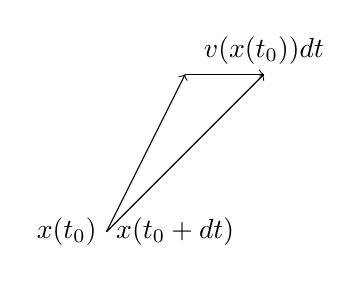
\begin{tikzpicture}
\draw[->] (0,0)node[left]{$x(t_0)$} -- (1,2);
\draw[->] (1,2) -- (2,2) node[above]{$v(x(t_0))dt$};
\draw[->] (0,0)node[right]{$x(t_0 +dt)$} -- (2,2);
\end{tikzpicture}
(we were constructing the curve $x$ each infinitesimal time step at a time from the intial value $x(t_0)$)
Like in 1D what we really get is an equation involving a vector valued integral.
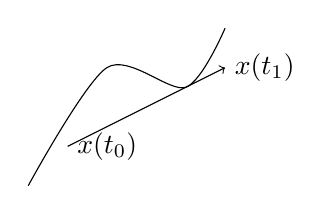
\begin{tikzpicture}
\draw plot[smooth] coordinates{(0,0)(1,1.5)(2,1.25)(2.5,2)};
\draw[->] (0.5,0.5) node[right]{$x(t_0)$} -- (2.5,1.5)node[right]{$x(t_1)$};
\end{tikzpicture}
But now we have a definition of the vector valued integral or the RHS.

\section{Separation of variables}
\subsection{Example: 1D} 
$v:R \rightarrow R$, $x \mapsto x$, $\dot{x} = x$, $x(0) = x_0$ (Initial Value Problem - IVP)\\
rewrite this as a differential equation:\\
$$\dot{x} = \frac{dx}{dt}$$
$$ dx = x(t + dt) - x(t) \underbrace{=}_{\text{K-L}} \dot{x}dt \underbrace{=}_{\text{ODE}} xdt \rightarrow dx = xdt$$
\begin{eqnarray*}
\frac{1}{x} dx = dt \underbrace{\rightsquigarrow}_{\text{Integrate}} \int_{x_0}^{x(t)} \frac{1}{x} dx &=& \int_{0}^{t} d\tau\\
&(=)& [lnx]_{x_0}^{x(t)} = [\tau]_{0}^{t}\\
&(=)& ln \frac{x(t)}{x_0} = t\\
&(=)& \frac{x(t)}{x_0} = e^t\\
&(=)& x(t) = x_0 e^t
\end{eqnarray*}
\underline{Check:}
$$\dot{x}(t) = x_0 e^t = x(t) \checkmark$$
$$x(0) = x_0 e^0 = x_0 \cdot t = x_0 \checkmark$$
If $x(0) = 0$ initially, $x(t) = 0$\\
\subsection{Method 1:} 
(separation of variables $v:R \rightarrow R$, $x \mapsto f(x)$, $f(x) = x$\\
\underline{Assume:} For each $x \leftarrow R$  $f(x)$ has a multiplicative inverse.
$$dx = f(x) dt \text{ (differential form of the ODE x = f(x))}$$
\begin{enumerate}
\item Separate the variables $x$ and $t$ $$\frac{1}{f(x)} dx = dt$$
\item Integrate both sides (IVP $\dot{x} = f(x)$, $x(t_0) = x_0$) $$\int_{x_0}^{x_t} \frac{1}{f(x)} dx= \int_{t_0}^{t} dt= t - t_0$$
\item Solve this equation for $x(t)$.
\end{enumerate}
\subsection{\underline{Q:} Does the equation have a solution? Is this solution unique?}
$$G:R \rightarrow R, y \mapsto \int_{x_0}^{y} \frac{1}{f(x)}dx$$
$\rightsquigarrow$ the equation becomes $G(x(t)) = t - t_0$\\
We notice $$ G(x_0) = \int_{x_0}^{x_0} \frac{1}{f(x)} dx = 0$$ $$ t_0 - t_0 = 0$$
We have a solution for $ t_0 - t_0 = 0$:\\
$$G'(y) = \frac{1}{f(y)}$$
This is different for zero $\rightsquigarrow$ No stationary points.\\
$\rightarrow$ It is either increasing or decreasing  (won't change monotonicity).\\
$\rightarrow$ Will always be able to find solution and solution is unique as $G$ is one to one (locally, for $t$ close to $t_0$).
\subsection{Method 2:} 
$$v: R \times R \rightarrow R \text{(time dependent vector field)}  (x,t) \mapsto v(x,t) = f(x)g(t) \text{($g(t) = 1$ in method 1)}$$
\underline{Assumption:} $f(x)$ has a multiplicative inverse in $R$\\
Consider the IVP $\dot{x} = v(x,t), x(0) = x_0, \dot{x}(t) = v(x(t),t)$
\begin{enumerate}
\item $dx = v(x,t)dt = f(x)g(t)dt$
\item Separate the variables: $\frac{1}{f(x)} dx = g(t) dt$
\item Integrate $\int_{x_0}^{x(t)} \frac{1}{f(x)} dx = \int_{t_0}^{t} g(\tau) d \tau$\\
\end{enumerate} 
Solve for x(t)

\section{2nd Order ODEs}
$$\ddot{x} = F(x,\dot{x},t)$$
$$F: R^n x R^n \times R \rightarrow R^n$$
\subsection{\underline{Q:} How to make it relate to 1st order ODEs?}
\begin{equation*}
\text{is a system of two 1st order ODEs}
\begin{cases}
\dot{x} = v \leftarrow \text{introduce a `velocity'.}\\
\dot{v} = \ddot{x} = F(x,v,t)
\end{cases}
\end{equation*}
\subsection{\underline{Q:} How to turn this into \underline{one} 1st order ODE?}
$$\underbrace{\begin{pmatrix} \dot{x}\\ \dot{v} \end{pmatrix}}_{\dot{z}} = \underbrace{\begin{pmatrix} v \\ F(x,v,t) \end{pmatrix}}_{\tilde{F}(z,t)}$$
$$ z = \begin{pmatrix} x \\ v \end{pmatrix}, \tilde{F}:R^{2n} \times R \rightarrow R^{2n}, (z,t) \mapsto \begin{pmatrix} v \\ F(z,t) \end{pmatrix}$$
A solution: $z: R \rightarrow R^{2n}, t \mapsto z(t)$ of $\dot{z} = \tilde{F}(z,t)$\\
i.e. $$\begin{pmatrix} \dot{x}(t) \\ \dot{v}(t) \end{pmatrix} = \begin{pmatrix} v(t) \\ F(x(t), v(t), t) \end{pmatrix}$$
$$\rightsquigarrow \dot{x}(t) = v(t)$$ $$\dot{v}(t) = F(x(t), v(t), t)$$
$$\underbrace{\rightsquigarrow}_{\text{substitute } \dot{x} = v} \dot{v}(t) = \ddot{x}(t) = F(x(t), \dot{x}(t), t) \checkmark$$
\subsection{\underline{Example:} (Free Fall)}
$$\ddot{x} = -g, F:R \rightarrow R, x \mapsto -g \text{(constant)}$$
\begin{equation*}
\text{Systen if 1st order ODEs } \begin{pmatrix} \dot{x} \\ v \end{pmatrix} = \begin{pmatrix} v \\ - g \end{pmatrix}
\begin{cases}
\dot{x} = v (I)\\
\dot{v} = -g (II)
\end{cases}
\end{equation*}
Integrate: $$(I) v(t) - v(0) = -gt \rightsquigarrow v(t) = v(0) - gt$$
Substitute in $(I)$: $$\dot{x} = v(t) = v(0) - gt (w:R \times R \rightarrow R, (x,t) \mapsto v(0) - gt, \dot{x} = w(x,t))$$
Integrate: $$x(t) - x(0) = v(0) t - \frac{1}{2} gt^2$$ $$x(t) = x(0) + v(0)t - \frac{1}{2} gt^2$$
\subsection{\underline{Example:} Pendulum}
\begin{center}
\begin{tikzpicture}
\draw[dotted](5,0) -- (5,-5);
\draw ([shift=(30:3cm)]5,-4) arc (-30:-150:3cm);
\draw ([shift=(30:1cm)]5,-1) arc (-30:-90:1cm) node[left]{$\varphi$};
\draw (5,0) -- (6.5,-3.6) node[right]{$x$};
\draw[->] (6.5,-3.6) -- (6.27,-3)node[left]{$T$}node[right]{$l$}; \draw[->] (6.5,-3.6) -- (6.5,-4.5)node[left]{$W$};\draw[->](6.5,-3.6) -- (7,-4)node[right]{$F_c$};\draw[->](6.5,-3.6) -- (7,-4.5)node[below]{$W_{\bot}$};\draw[->](6.5,-3.6) -- (5.5,-4)node[left]{$W_{\parallel}$};
\end{tikzpicture}
\end{center}
(We ignore centripetal force due to constraint)\\
$T$ = tension\\
$F_c$ = centrifugal force\\
$W$ = weight\\
contraint: rod is rigid\\
$\rightsquigarrow$ bob of mass $m$ is going to move on  a circle of radius $l$.\\ 
$\rightsquigarrow$ resulting force: $$W_{\parallel} =  - mg sin \varphi$$  $$m\ddot{x} = W_{\parallel} =  - mg sin \varphi$$ (use $ x = \varphi l$) $$\ddot{x} = \ddot{\varphi} l = - g sin \varphi$$ $$\rightsquigarrow \ddot{\varphi} = - \frac{g}{l} sin \varphi $$
Step 1 $\rightarrow$ rewrite this as a system of 1st order ODEs: $$\phi = \nu$$ $$ \dot{\nu} = - \frac{g}{l} sin \varphi $$
Try separation of variables:
$$d \nu = \frac{-g}{l} sin \varphi dt, d \varphi = \nu dt$$
Doesn't work as per method. Try further:
$$dt = \frac{d \varphi}{\nu} \text{( careful $\nu = 0$ is possible)}$$
$$\rightsquigarrow d\nu =\frac{-g}{l} sin \varphi \frac{d \varphi}{\nu}$$
Now we can separate: $$\nu d\nu = -\frac{g}{l} sin \varphi d \varphi $$
(We have lost the time variable) Integrate: $$\int_{\nu(\varphi_0)}^{\nu(\varphi)} \nu d \nu = -\frac{g}{l}\int_{\nu(\varphi_0)}^{\nu(\varphi)} sin \varphi d \varphi$$
($\varphi_0$ - pulled up the bob an angle of $\varphi_0$ and release from rest $\nu(\varphi_0) = 0$)
$$\rightsquigarrow \frac{1}{2} \nu (\varphi)^2 = \frac{g}{l}(cos \varphi - cos \varphi_0)$$
$$(=) \nu(\varphi) = \sqrt{\frac{2g}{l}(cos \varphi - cos \varphi_0)}$$
\subsection{\underline{Q:} What have we figured out?}
We found the angular velocity as a function of the angle not the time.\\
This gives us an ODE: $$\dot{\varphi} = \nu(\varphi) = \sqrt{\frac{2g}{l}(cos \varphi - cos \varphi_0)}$$
(Apply separation of variables:)$$\frac{1}{\sqrt{\frac{2g}{l}(cos \varphi - cos \varphi_0)}} d \varphi = dt$$
$$\sqrt{\frac{1}{2g}} \int_{\varphi_0}^{\varphi(t)} \frac{1}{\sqrt{cos \varphi - cos \varphi_0}} d \varphi = t$$
Solve for t: (problem: this is an integral that has not got an elementary function as an antiderivative)\\
$$E(z) = \int_{\varphi_0}^{z} \frac{1}{\sqrt{cos \varphi - cos \varphi_0}} d \varphi \text{(eliptic integral)}$$


\end{document}